\documentclass{article}
\usepackage[a4paper, left = 25mm, right = 25mm, bottom = 25mm]{geometry}
\usepackage{amsmath}
\usepackage{graphicx}
\usepackage{float}
\usepackage{hyperref}
\usepackage{fancyvrb}
\usepackage{matlab-prettifier}
\usepackage{enumitem}
\usepackage{color}
% \usepackage{minted}
\usepackage{palatino}
\fontfamily{SansSerif}

\setlength{\parindent}{0pt}

\title{EE324: Control Systems Lab \\ Experiment 2: Inverted Pendulum\\ \textbf{Group 1 - Thursday}}
\author{\large Harsh S Roniyar\\ \large 22B3942 \and \large Pranav Prakash\\ \large 22B3945 \and \large Aman Verma\\ \large 22B3929}

\begin{document}

\maketitle

\section{Objective}
To design and implement control action for maintaining a pendulum in the upright position (even when subjected to external disturbances) through LQR technique in an Arduino Mega.
\vspace{5pt}

The specific objectives were:
\begin{itemize}[noitemsep]
\item To restrict the pendulum arm vibration ($\alpha$) within $\pm 3^{\circ}$. 
\item To restrict the base angle oscillation ($\theta$) within $\pm 30^{\circ}$. 
\end{itemize}

\section{Control Algorithm}

The control algorithm used in this experiment is Linear Quadratic Regulator (LQR). 
Given the plant model
\begin{equation}
  \dot x(t) = Ax(t) + Bu(t)
\end{equation}
where $x(t)$ is the state vector, $u(t)$ is the control input, $A$ is the state matrix and $B$ is the input matrix. The objective of the Linear Quadratic Regulator (LQR) problem is to find the control input $u(t)$ that minimizes the cost function J given by - 
\begin{equation}
  J = \int_{0}^{\infty} (x^T(t)Qx(t) + u^T(t)Ru(t)) \text{d}t
\end{equation}  
where $Q$ and $R$ are positive definite matrices. The control input $u(t)$ is given by the feedback law -
\begin{equation}
  u(t) = -Kx(t)
\end{equation}
where $K$ is the state feedback gain matrix given by -
\begin{equation}
  K = R^{-1}B^TP
\end{equation}
and $P$ is the solution to the equation - %Riccati equation
\begin{equation}
  A^TP + PA + Q - PBR^{-1}B^TP = 0
\end{equation}

\clearpage

Some important code snippets showing the implementation of the LQR controller in Arduino.
\begin{lstlisting}[style=Matlab-Pyglike, breaklines=true,postbreak=\mbox{\textcolor{red}{$\hookrightarrow$}\space}, language=C++, escapeinside={(*@}{@*)}]
/*
  Experiment 2 : Inverted Pendulum

  Group 1:
  22B3929 - Aman Verma
  22B3942 - Harsh S Roniyar
  22B3945 - Pranav Prakash
*/

/*
Q = [410, 0, 0, 0;
    0,4, 0, 0;
    0, 0, 50, 0;
    0, 0, 0, 100];
R = 14;
*/

#include <SPI.h>

/* Serial rates for UART */
#define BAUDRATE        115200

/* SPI commands */
#define AMT22_NOP       0x00
#define AMT22_RESET     0x60
#define AMT22_ZERO      0x70

/* Define special ascii characters */
#define NEWLINE         0x0A
#define TAB             0x09

/* We will use these define macros so we can write code once compatible with 12 or 14 bit encoders */
#define RES12           12
#define RES14           14

/* SPI pins */
#define ENC_0            2
#define ENC_1            3
#define SPI_MOSI        51
#define SPI_MISO        50
#define SPI_SCLK        52

void setup()
{
  (*@{\raisebox{-1pt}[0pt][0pt]{$\vdots$}}@*)
}

void loop()
{
  uint16_t encoderPosition0, encoderPosition1;
  uint8_t attempts;
  float theta, alpha;
  float start_pos_arm = (float)getPositionSPI(ENC_0, RES14)*360/16383;
  float error_pendulum_cur,error_arm_cur, error_pendulum_prev,error_arm_prev, velocity_arm, velocity_pendulum, Vm_out;
  int fbsignal;
  float k[4] = {-5.41162769282160,  96.7114158315394,  -3.49111501865230, 13.0618707845219};

  encoderPosition1 = getPositionSPI(ENC_1, RES14);
  encoderPosition0 = getPositionSPI(ENC_0, RES14);
  
  theta = (float)encoderPosition0*360/16383;
  alpha = (float)encoderPosition1*360/16383;

  error_pendulum_prev = alpha - 180;
  error_arm_prev = theta - start_pos_arm;
  while(1){
   
    encoderPosition0 = getPositionSPI(ENC_0, RES14);
    encoderPosition1 = getPositionSPI(ENC_1, RES14);
   
    theta = (float)encoderPosition0*360/16383;
    alpha = (float)encoderPosition1*360/16383;
   
    error_pendulum_cur = alpha - 180;
    error_arm_cur = theta - start_pos_arm;
    velocity_pendulum = (error_pendulum_cur - error_pendulum_prev)/0.025;
    velocity_arm = (error_arm_cur - error_arm_prev)/0.025;
    //LQR CODE
    Vm_out = (k[0]*error_arm_cur + k[1]*error_pendulum_cur + k[2]*velocity_arm + k[3]*velocity_pendulum)*3.1415926535/180;
    
    fbsignal =map(abs(Vm_out),0,12,0,255);

    Serial.print("arm_error: ");
    Serial.print(error_arm_cur);
    Serial.print("pendulum_error: ");
    Serial.println(error_pendulum_cur);

    if(Vm_out>0){
      analogWrite(12, constrain(fbsignal,0,255));  // Set motor direction
      analogWrite(13, 0);
    }
    else{
      analogWrite(13, constrain(fbsignal,0,255));  // Set motor direction
      analogWrite(12, 0);
    }

    error_pendulum_prev = error_pendulum_cur;
    error_arm_prev=error_arm_cur;
    delay(25);
  }
}

\end{lstlisting}

% \clearpage
\section{Challenges Faced and Solutions}
\begin{itemize}%[nolistsep]
    \item \textbf{Tuning of the LQR Controller:} Finding the appropriate values for the LQR controllables ($Q$, $R$) to meet the design specifications ($K$) was challenging.\\
    \underline{\textit{Solution:}} Started with smaller values of $Q$ and $R$ and gradually increased them to meet the design specifications. Monitored the system's response closely using \textbf{MATLAB} during tuning to prevent instability.

    \item \textbf{Attaining Controller Objectives:} Achieving a balance between a fast response (stabilization) and restricting pendulum vibration ($\alpha$) within $\pm 3^{\circ}$ and base angle oscillation ($\theta$) within $\pm 30^{\circ}$ was challenging. Over-tuning for speed lead to excessive overshoot or instability.\\
    \underline{\textit{Solution:}} Adjusted the values of $Q$ and $R$ to satisfy the constraints. Monitored the system's response closely using Serial Plotter and its resilience to external disturbance during tuning. The step response plot obtained from \textbf{MATLAB} is shown in Figure \ref{fig:step}.
    \begin{figure}[!htb]
        \centering
        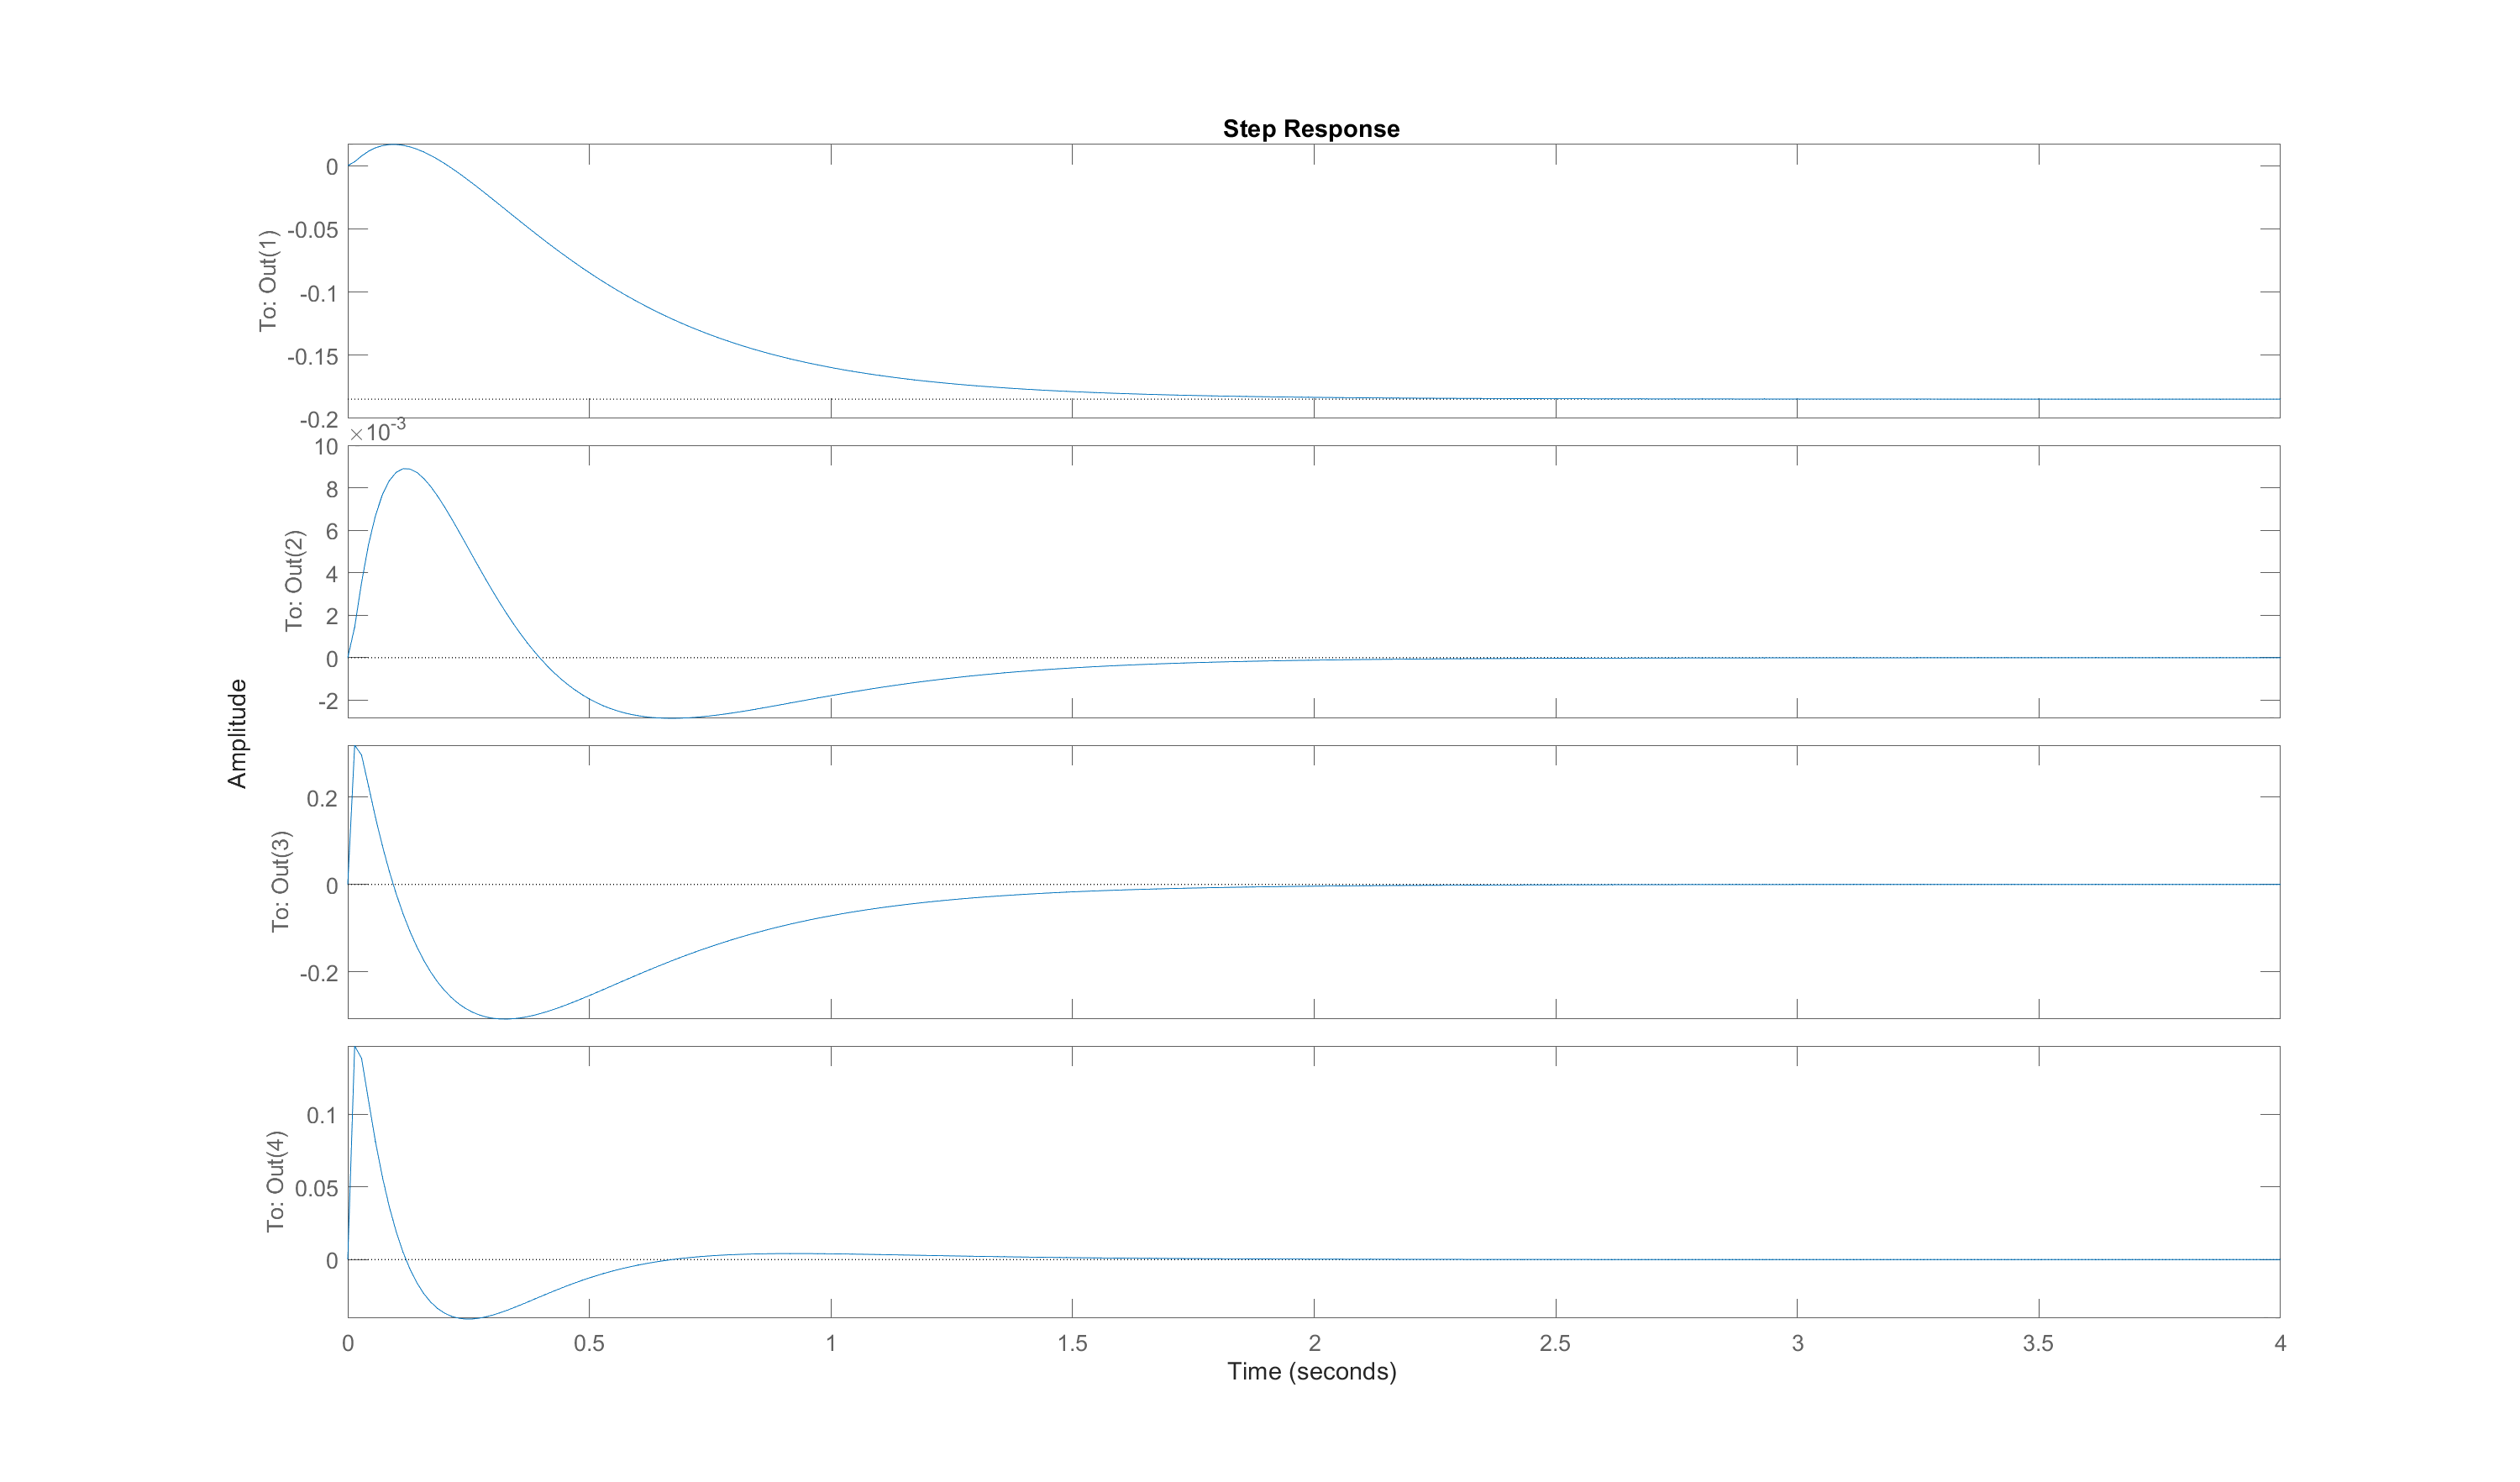
\includegraphics[width=\textwidth]{../././step_response.png}
        \caption{Step Response of the System}
        \label{fig:step}
    \end{figure}
    \vspace{-10pt}
\end{itemize}

\section{Results}

\begin{itemize}[nolistsep]
    \item The final values of the LQR controllables were found to be $$Q = \begin{bmatrix} 410 & 0 & 0 & 0 \\ 0 & 4 & 0 & 0 \\ 0 & 0 & 50 & 0 \\ 0 & 0 & 0 & 100 \end{bmatrix}$$ $$R = 14$$
    \vspace{-10pt}
    \item The feedback gain matrix $K$ was found to be $$K = \begin{bmatrix} -5.41 & 96.71 & -3.49 & 13.06 \end{bmatrix}$$
    \item The relative arm and pendulum position (error) vs time plot is shown in Figure \ref{fig:plot}
    \vspace{-10pt}
    \begin{figure}[!htb]
        \centering
        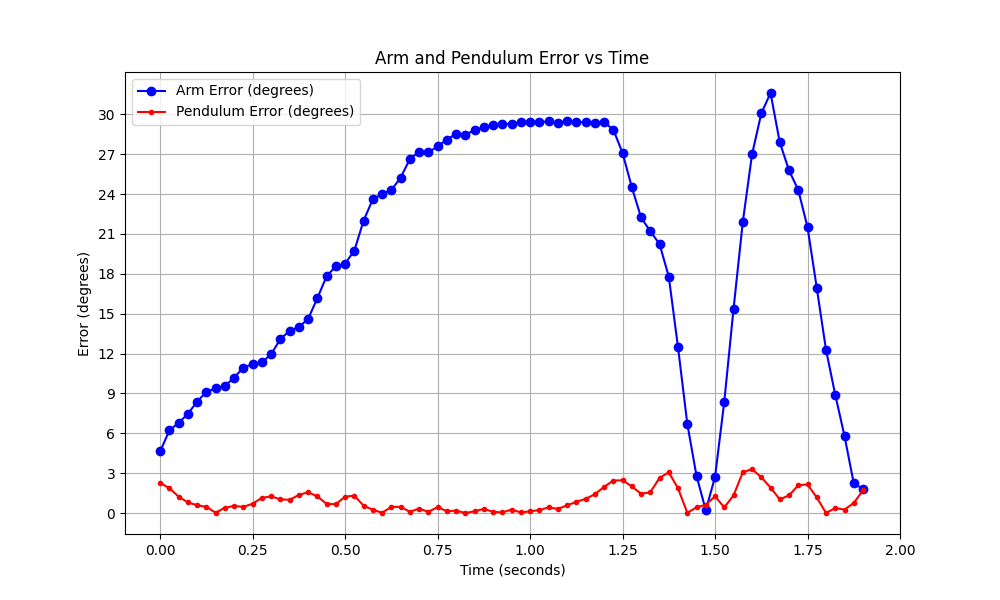
\includegraphics[width=0.8\textwidth]{../././inv_pendulum.png}
        \caption{Relative Position vs Time}
        \label{fig:plot}
    \end{figure}
\end{itemize}

\section{Observations and Inference}
\begin{itemize}[nolistsep]
    \item The LQR controller was able to stabilize the inverted pendulum system within desired constraints.
    \item The system was able to maintain the pendulum arm within $\pm 3^{\circ}$ and the base angle within $\pm 30^{\circ}$ as can be seen in the plot \ref{fig:plot}.
    \item The system recovered from external disturbances and maintain stability when displaced from the equilibrium position.
\end{itemize}

% \section{TA Result Sheet}

% \begin{center}
%     \includegraphics[width=0.8\textwidth]{../././TASheet.jpg}
% \end{center}

\end{document}